\documentclass[11pt]{article}
\usepackage[T1]{fontenc}
\usepackage[margin=1in]{geometry}
\usepackage{amsmath,amssymb,amsthm}
\usepackage{graphicx}
\usepackage{booktabs}

\newtheorem{theorem}{Theorem}

\title{Energy Decay in a Damped Harmonic Oscillator}
\author{Lena Ortiz\\ \small Department of Physics, Northfield College}
\date{October 2026}

\begin{document}
\maketitle

\begin{abstract}
We study the free motion of a mass on a linear spring subject to viscous
damping. We derive the closed-form solution in the underdamped regime, show
that the mechanical energy decays monotonically, and compare the analytic
solution with two simple numerical schemes.
\end{abstract}

\section{Introduction}

The damped harmonic oscillator is the simplest model of a system that loses
energy to its surroundings~\cite{goldstein}. Its equation of motion is
\begin{equation}\label{eq:motion}
  m\ddot{x} + c\dot{x} + kx = 0,
\end{equation}
where $m>0$ is the mass, $c \ge 0$ the damping coefficient and $k>0$ the
spring constant.\footnote{All quantities are in SI units.} Dividing by $m$
and writing $\omega_0 = \sqrt{k/m}$ and $\gamma = c/(2m)$ gives the
\emph{standard form}
\begin{equation}\label{eq:standard}
  \ddot{x} + 2\gamma\dot{x} + \omega_0^2 x = 0.
\end{equation}

\section{Solution}

Substituting $x = e^{\lambda t}$ into~\eqref{eq:standard} gives the
characteristic equation $\lambda^2 + 2\gamma\lambda + \omega_0^2 = 0$, whose
roots are
\begin{equation}\label{eq:roots}
  \lambda_{\pm} = -\gamma \pm \sqrt{\gamma^2 - \omega_0^2}.
\end{equation}
The behaviour depends on the sign of the discriminant:
\[
  \text{regime} =
  \begin{cases}
    \text{underdamped}, & \gamma < \omega_0,\\
    \text{critically damped}, & \gamma = \omega_0,\\
    \text{overdamped}, & \gamma > \omega_0.
  \end{cases}
\]
In the underdamped case let $\omega_d = \sqrt{\omega_0^2 - \gamma^2}$. With
$x(0) = x_0$ and $\dot{x}(0) = 0$ the solution is
\begin{equation}\label{eq:solution}
  x(t) = x_0\, e^{-\gamma t}\left(\cos\omega_d t
         + \frac{\gamma}{\omega_d}\sin\omega_d t\right).
\end{equation}
Equivalently, with $\mathbf{y} = (x, \dot{x})^{\mathsf{T}}$,
equation~\eqref{eq:standard} becomes the first-order system
\begin{equation}\label{eq:system}
  \dot{\mathbf{y}} =
  \begin{pmatrix} 0 & 1 \\ -\omega_0^2 & -2\gamma \end{pmatrix}\mathbf{y}.
\end{equation}

\begin{theorem}
The energy $E(t) = \tfrac12 m\dot{x}^2 + \tfrac12 kx^2$ never increases. More
precisely, $\dfrac{dE}{dt} = -c\,\dot{x}^2 \le 0$.
\end{theorem}

\begin{proof}
Differentiate $E$ and use~\eqref{eq:motion}:
\begin{align*}
  \frac{dE}{dt} &= m\dot{x}\ddot{x} + kx\dot{x} \\
                &= \dot{x}\,(m\ddot{x} + kx) = -c\,\dot{x}^2. \qedhere
\end{align*}
\end{proof}

\section{Numerical check}

We integrated~\eqref{eq:standard} with $\omega_0 = 2$, $\gamma = 0.2$ and
$x_0 = 1$ on $t \in [0, 10]$, using the explicit Euler method and the
classical fourth-order Runge--Kutta method (RK4)~\cite{hairer}. For each step
size $h$ we:
\begin{enumerate}
  \item integrated from $t=0$ to $t=10$ with $10/h$ steps;
  \item compared every step with the exact solution~\eqref{eq:solution};
  \item recorded the largest absolute difference.
\end{enumerate}
Table~\ref{tab:errors} lists the results and Figure~\ref{fig:solution} shows
the exact solution.

\begin{table}[h]
  \centering
  \caption{Maximum absolute error on $[0, 10]$.}
  \label{tab:errors}
  \begin{tabular}{ccc}
    \toprule
    Step $h$ & Euler & RK4 \\
    \midrule
    $0.100$ & $8.51 \times 10^{-1}$ & $5.00 \times 10^{-5}$ \\
    $0.050$ & $2.50 \times 10^{-1}$ & $3.10 \times 10^{-6}$ \\
    $0.025$ & $1.06 \times 10^{-1}$ & $1.93 \times 10^{-7}$ \\
    \bottomrule
  \end{tabular}
\end{table}

\begin{figure}[h]
  \centering
  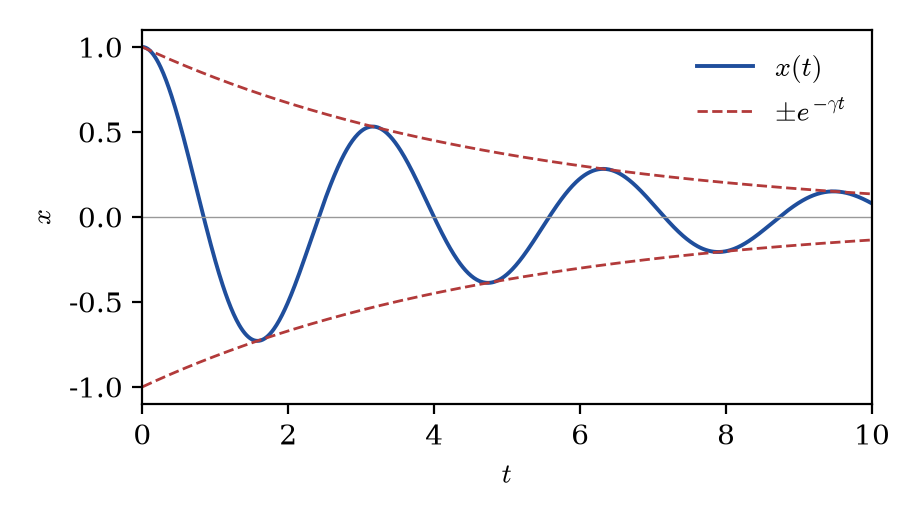
\includegraphics[width=0.62\textwidth]{fig1.png}
  \caption{The solution~\eqref{eq:solution} for $\gamma = 0.2$,
    $\omega_0 = 2$ and its envelope $\pm e^{-\gamma t}$.}
  \label{fig:solution}
\end{figure}

Two things stand out:
\begin{itemize}
  \item Euler's error is large because the method \textbf{adds} energy at
        every step, which works against the physical damping.
  \item Halving $h$ divides the RK4 error by about $16 = 2^4$, as expected
        for a fourth-order method.
\end{itemize}

\begin{thebibliography}{9}
\bibitem{goldstein}
  H.~Goldstein, C.~Poole and J.~Safko,
  \emph{Classical Mechanics}, 3rd ed., Addison-Wesley, 2002.
\bibitem{hairer}
  E.~Hairer, S.~P.~N{\o}rsett and G.~Wanner,
  \emph{Solving Ordinary Differential Equations~I}, 2nd ed., Springer, 1993.
\end{thebibliography}

\end{document}
